\documentclass[12pt]{article}
%%\usepackage[T1]{fontenc}
\usepackage[dvipsnames]{xcolor}
%\usepackage{bigfoot} % to allow verbatim in footnote
\usepackage[numbered,framed]{matlab-prettifier}
\usepackage[letterpaper, margin=1in]{geometry}

\usepackage[T1]{fontenc}
% Nicer default font (+ math font) than Computer Modern for most use cases
\usepackage{mathpazo}

% Basic figure setup, for now with no caption control since it's done
% automatically by Pandoc (which extracts ![](path) syntax from Markdown).
\usepackage{graphicx}
% We will generate all images so they have a width \maxwidth. This means
% that they will get their normal width if they fit onto the page, but
% are scaled down if they would overflow the margins.
\makeatletter
\def\maxwidth{\ifdim\Gin@nat@width>\linewidth\linewidth
	\else\Gin@nat@width\fi}
\makeatother
\let\Oldincludegraphics\includegraphics
% Set max figure width to be 80% of text width, for now hardcoded.
\renewcommand{\includegraphics}[1]{\Oldincludegraphics[width=.8\maxwidth]{#1}}
% Ensure that by default, figures have no caption (until we provide a
% proper Figure object with a Caption API and a way to capture that
% in the conversion process - todo).
\usepackage{caption}
\DeclareCaptionLabelFormat{nolabel}{}
\captionsetup{labelformat=nolabel}

\usepackage{adjustbox} % Used to constrain images to a maximum size 
\usepackage{xcolor} % Allow colors to be defined
\usepackage{enumerate} % Needed for markdown enumerations to work
\usepackage{geometry} % Used to adjust the document margins
\usepackage{amsmath} % Equations
\usepackage{amssymb} % Equations
\usepackage{textcomp} % defines textquotesingle
% Hack from http://tex.stackexchange.com/a/47451/13684:
\AtBeginDocument{%
	\def\PYZsq{\textquotesingle}% Upright quotes in Pygmentized code
}
\usepackage{upquote} % Upright quotes for verbatim code
\usepackage{eurosym} % defines \euro
\usepackage[mathletters]{ucs} % Extended unicode (utf-8) support
\usepackage[utf8x]{inputenc} % Allow utf-8 characters in the tex document
\usepackage{fancyvrb} % verbatim replacement that allows latex
\usepackage{grffile} % extends the file name processing of package graphics 
% to support a larger range 
% The hyperref package gives us a pdf with properly built
% internal navigation ('pdf bookmarks' for the table of contents,
% internal cross-reference links, web links for URLs, etc.)
\usepackage{hyperref}
\usepackage{longtable} % longtable support required by pandoc >1.10
\usepackage{booktabs}  % table support for pandoc > 1.12.2
\usepackage[inline]{enumitem} % IRkernel/repr support (it uses the enumerate* environment)
\usepackage[normalem]{ulem} % ulem is needed to support strikethroughs (\sout)
% normalem makes italics be italics, not underlines
\usepackage{mathrsfs}

\usepackage{amsmath, amssymb, amsthm}
\usepackage{fancyhdr}
\usepackage{mathtools}
\usepackage{tikz}
\usepackage{enumerate}
\usepackage{microtype}
\usepackage[english]{babel}
%\usepackage[utf8]{inputenc}
\usepackage{cancel}
\usepackage{titlesec}
\usepackage{xfrac}
\usepackage{marginnote}
%\usepackage [autostyle, english = american]{csquotes}
%\MakeOuterQuote{"}
\usepackage{filecontents}
\usepackage{fancyvrb}



\pagestyle{fancy}
\rhead{Oscar Martinez}
\lhead{STA 5106} 					%Insert subject
\chead{HW 3: Problems 1-3} 					%Insert Title

\newtheorem{theorem}{Theorem}[section]

\newcommand{\Real}{\mathbb{R}}
\newcommand{\Prob}{\mathbb{P}}
\newcommand{\Lagr}{\mathcal{L}}
\newcommand{\LRA}{\Leftrightarrow}
\newcommand{\LA}{\Leftarrow}
\newcommand{\RA}{\Rightarrow}
\newcommand{\ra}{\rightarrow}
\newcommand{\rsa}{\rightsquigarrow} 
\newcommand\Ccancel[2][black]{\renewcommand\CancelColor{\color{#1}}\cancel{#2}}
\newcommand{\at}{a_{t+1}}
\newcommand{\ct}{c_{t+1}}
\DeclareMathOperator{\EX}{\mathbb{E}}% expected value
\DeclareMathOperator{\Var}{\mathbb{V}}% expected value

\renewcommand{\footrulewidth}{0.2pt}
\renewcommand{\qedsymbol}{$\blacksquare$}
\renewcommand{\thesection}{\arabic{section}.}
\renewcommand{\thesubsection}{(\alph{subsection})}
\renewcommand{\thesubsubsection}{\roman{subsubsection}.)}

 % Colors for the hyperref package
\definecolor{urlcolor}{rgb}{0,.145,.698}
\definecolor{linkcolor}{rgb}{.71,0.21,0.01}
\definecolor{citecolor}{rgb}{.12,.54,.11}

% ANSI colors
\definecolor{ansi-black}{HTML}{3E424D}
\definecolor{ansi-black-intense}{HTML}{282C36}
\definecolor{ansi-red}{HTML}{E75C58}
\definecolor{ansi-red-intense}{HTML}{B22B31}
\definecolor{ansi-green}{HTML}{00A250}
\definecolor{ansi-green-intense}{HTML}{007427}
\definecolor{ansi-yellow}{HTML}{DDB62B}
\definecolor{ansi-yellow-intense}{HTML}{B27D12}
\definecolor{ansi-blue}{HTML}{208FFB}
\definecolor{ansi-blue-intense}{HTML}{0065CA}
\definecolor{ansi-magenta}{HTML}{D160C4}
\definecolor{ansi-magenta-intense}{HTML}{A03196}
\definecolor{ansi-cyan}{HTML}{60C6C8}
\definecolor{ansi-cyan-intense}{HTML}{258F8F}
\definecolor{ansi-white}{HTML}{C5C1B4}
\definecolor{ansi-white-intense}{HTML}{A1A6B2}
\definecolor{ansi-default-inverse-fg}{HTML}{FFFFFF}
\definecolor{ansi-default-inverse-bg}{HTML}{000000}

% commands and environments needed by pandoc snippets
% extracted from the output of `pandoc -s`
\providecommand{\tightlist}{%
	\setlength{\itemsep}{0pt}\setlength{\parskip}{0pt}}
\DefineVerbatimEnvironment{Highlighting}{Verbatim}{commandchars=\\\{\}}
% Add ',fontsize=\small' for more characters per line
\newenvironment{Shaded}{}{}
\newcommand{\KeywordTok}[1]{\textcolor[rgb]{0.00,0.44,0.13}{\textbf{{#1}}}}
\newcommand{\DataTypeTok}[1]{\textcolor[rgb]{0.56,0.13,0.00}{{#1}}}
\newcommand{\DecValTok}[1]{\textcolor[rgb]{0.25,0.63,0.44}{{#1}}}
\newcommand{\BaseNTok}[1]{\textcolor[rgb]{0.25,0.63,0.44}{{#1}}}
\newcommand{\FloatTok}[1]{\textcolor[rgb]{0.25,0.63,0.44}{{#1}}}
\newcommand{\CharTok}[1]{\textcolor[rgb]{0.25,0.44,0.63}{{#1}}}
\newcommand{\StringTok}[1]{\textcolor[rgb]{0.25,0.44,0.63}{{#1}}}
\newcommand{\CommentTok}[1]{\textcolor[rgb]{0.38,0.63,0.69}{\textit{{#1}}}}
\newcommand{\OtherTok}[1]{\textcolor[rgb]{0.00,0.44,0.13}{{#1}}}
\newcommand{\AlertTok}[1]{\textcolor[rgb]{1.00,0.00,0.00}{\textbf{{#1}}}}
\newcommand{\FunctionTok}[1]{\textcolor[rgb]{0.02,0.16,0.49}{{#1}}}
\newcommand{\RegionMarkerTok}[1]{{#1}}
\newcommand{\ErrorTok}[1]{\textcolor[rgb]{1.00,0.00,0.00}{\textbf{{#1}}}}
\newcommand{\NormalTok}[1]{{#1}}

% Additional commands for more recent versions of Pandoc
\newcommand{\ConstantTok}[1]{\textcolor[rgb]{0.53,0.00,0.00}{{#1}}}
\newcommand{\SpecialCharTok}[1]{\textcolor[rgb]{0.25,0.44,0.63}{{#1}}}
\newcommand{\VerbatimStringTok}[1]{\textcolor[rgb]{0.25,0.44,0.63}{{#1}}}
\newcommand{\SpecialStringTok}[1]{\textcolor[rgb]{0.73,0.40,0.53}{{#1}}}
\newcommand{\ImportTok}[1]{{#1}}
\newcommand{\DocumentationTok}[1]{\textcolor[rgb]{0.73,0.13,0.13}{\textit{{#1}}}}
\newcommand{\AnnotationTok}[1]{\textcolor[rgb]{0.38,0.63,0.69}{\textbf{\textit{{#1}}}}}
\newcommand{\CommentVarTok}[1]{\textcolor[rgb]{0.38,0.63,0.69}{\textbf{\textit{{#1}}}}}
\newcommand{\VariableTok}[1]{\textcolor[rgb]{0.10,0.09,0.49}{{#1}}}
\newcommand{\ControlFlowTok}[1]{\textcolor[rgb]{0.00,0.44,0.13}{\textbf{{#1}}}}
\newcommand{\OperatorTok}[1]{\textcolor[rgb]{0.40,0.40,0.40}{{#1}}}
\newcommand{\BuiltInTok}[1]{{#1}}
\newcommand{\ExtensionTok}[1]{{#1}}
\newcommand{\PreprocessorTok}[1]{\textcolor[rgb]{0.74,0.48,0.00}{{#1}}}
\newcommand{\AttributeTok}[1]{\textcolor[rgb]{0.49,0.56,0.16}{{#1}}}
\newcommand{\InformationTok}[1]{\textcolor[rgb]{0.38,0.63,0.69}{\textbf{\textit{{#1}}}}}
\newcommand{\WarningTok}[1]{\textcolor[rgb]{0.38,0.63,0.69}{\textbf{\textit{{#1}}}}}


% Define a nice break command that doesn't care if a line doesn't already
% exist.
\def\br{\hspace*{\fill} \\* }
% Math Jax compatibility definitions
\def\gt{>}
\def\lt{<}
\let\Oldtex\TeX
\let\Oldlatex\LaTeX
\renewcommand{\TeX}{\textrm{\Oldtex}}
\renewcommand{\LaTeX}{\textrm{\Oldlatex}}
% Document parameters
% Document title
 % Pygments definitions

\makeatletter
\def\PY@reset{\let\PY@it=\relax \let\PY@bf=\relax%
	\let\PY@ul=\relax \let\PY@tc=\relax%
	\let\PY@bc=\relax \let\PY@ff=\relax}
\def\PY@tok#1{\csname PY@tok@#1\endcsname}
\def\PY@toks#1+{\ifx\relax#1\empty\else%
	\PY@tok{#1}\expandafter\PY@toks\fi}
\def\PY@do#1{\PY@bc{\PY@tc{\PY@ul{%
				\PY@it{\PY@bf{\PY@ff{#1}}}}}}}
\def\PY#1#2{\PY@reset\PY@toks#1+\relax+\PY@do{#2}}

\expandafter\def\csname PY@tok@w\endcsname{\def\PY@tc##1{\textcolor[rgb]{0.73,0.73,0.73}{##1}}}
\expandafter\def\csname PY@tok@c\endcsname{\let\PY@it=\textit\def\PY@tc##1{\textcolor[rgb]{0.25,0.50,0.50}{##1}}}
\expandafter\def\csname PY@tok@cp\endcsname{\def\PY@tc##1{\textcolor[rgb]{0.74,0.48,0.00}{##1}}}
\expandafter\def\csname PY@tok@k\endcsname{\let\PY@bf=\textbf\def\PY@tc##1{\textcolor[rgb]{0.00,0.50,0.00}{##1}}}
\expandafter\def\csname PY@tok@kp\endcsname{\def\PY@tc##1{\textcolor[rgb]{0.00,0.50,0.00}{##1}}}
\expandafter\def\csname PY@tok@kt\endcsname{\def\PY@tc##1{\textcolor[rgb]{0.69,0.00,0.25}{##1}}}
\expandafter\def\csname PY@tok@o\endcsname{\def\PY@tc##1{\textcolor[rgb]{0.40,0.40,0.40}{##1}}}
\expandafter\def\csname PY@tok@ow\endcsname{\let\PY@bf=\textbf\def\PY@tc##1{\textcolor[rgb]{0.67,0.13,1.00}{##1}}}
\expandafter\def\csname PY@tok@nb\endcsname{\def\PY@tc##1{\textcolor[rgb]{0.00,0.50,0.00}{##1}}}
\expandafter\def\csname PY@tok@nf\endcsname{\def\PY@tc##1{\textcolor[rgb]{0.00,0.00,1.00}{##1}}}
\expandafter\def\csname PY@tok@nc\endcsname{\let\PY@bf=\textbf\def\PY@tc##1{\textcolor[rgb]{0.00,0.00,1.00}{##1}}}
\expandafter\def\csname PY@tok@nn\endcsname{\let\PY@bf=\textbf\def\PY@tc##1{\textcolor[rgb]{0.00,0.00,1.00}{##1}}}
\expandafter\def\csname PY@tok@ne\endcsname{\let\PY@bf=\textbf\def\PY@tc##1{\textcolor[rgb]{0.82,0.25,0.23}{##1}}}
\expandafter\def\csname PY@tok@nv\endcsname{\def\PY@tc##1{\textcolor[rgb]{0.10,0.09,0.49}{##1}}}
\expandafter\def\csname PY@tok@no\endcsname{\def\PY@tc##1{\textcolor[rgb]{0.53,0.00,0.00}{##1}}}
\expandafter\def\csname PY@tok@nl\endcsname{\def\PY@tc##1{\textcolor[rgb]{0.63,0.63,0.00}{##1}}}
\expandafter\def\csname PY@tok@ni\endcsname{\let\PY@bf=\textbf\def\PY@tc##1{\textcolor[rgb]{0.60,0.60,0.60}{##1}}}
\expandafter\def\csname PY@tok@na\endcsname{\def\PY@tc##1{\textcolor[rgb]{0.49,0.56,0.16}{##1}}}
\expandafter\def\csname PY@tok@nt\endcsname{\let\PY@bf=\textbf\def\PY@tc##1{\textcolor[rgb]{0.00,0.50,0.00}{##1}}}
\expandafter\def\csname PY@tok@nd\endcsname{\def\PY@tc##1{\textcolor[rgb]{0.67,0.13,1.00}{##1}}}
\expandafter\def\csname PY@tok@s\endcsname{\def\PY@tc##1{\textcolor[rgb]{0.73,0.13,0.13}{##1}}}
\expandafter\def\csname PY@tok@sd\endcsname{\let\PY@it=\textit\def\PY@tc##1{\textcolor[rgb]{0.73,0.13,0.13}{##1}}}
\expandafter\def\csname PY@tok@si\endcsname{\let\PY@bf=\textbf\def\PY@tc##1{\textcolor[rgb]{0.73,0.40,0.53}{##1}}}
\expandafter\def\csname PY@tok@se\endcsname{\let\PY@bf=\textbf\def\PY@tc##1{\textcolor[rgb]{0.73,0.40,0.13}{##1}}}
\expandafter\def\csname PY@tok@sr\endcsname{\def\PY@tc##1{\textcolor[rgb]{0.73,0.40,0.53}{##1}}}
\expandafter\def\csname PY@tok@ss\endcsname{\def\PY@tc##1{\textcolor[rgb]{0.10,0.09,0.49}{##1}}}
\expandafter\def\csname PY@tok@sx\endcsname{\def\PY@tc##1{\textcolor[rgb]{0.00,0.50,0.00}{##1}}}
\expandafter\def\csname PY@tok@m\endcsname{\def\PY@tc##1{\textcolor[rgb]{0.40,0.40,0.40}{##1}}}
\expandafter\def\csname PY@tok@gh\endcsname{\let\PY@bf=\textbf\def\PY@tc##1{\textcolor[rgb]{0.00,0.00,0.50}{##1}}}
\expandafter\def\csname PY@tok@gu\endcsname{\let\PY@bf=\textbf\def\PY@tc##1{\textcolor[rgb]{0.50,0.00,0.50}{##1}}}
\expandafter\def\csname PY@tok@gd\endcsname{\def\PY@tc##1{\textcolor[rgb]{0.63,0.00,0.00}{##1}}}
\expandafter\def\csname PY@tok@gi\endcsname{\def\PY@tc##1{\textcolor[rgb]{0.00,0.63,0.00}{##1}}}
\expandafter\def\csname PY@tok@gr\endcsname{\def\PY@tc##1{\textcolor[rgb]{1.00,0.00,0.00}{##1}}}
\expandafter\def\csname PY@tok@ge\endcsname{\let\PY@it=\textit}
\expandafter\def\csname PY@tok@gs\endcsname{\let\PY@bf=\textbf}
\expandafter\def\csname PY@tok@gp\endcsname{\let\PY@bf=\textbf\def\PY@tc##1{\textcolor[rgb]{0.00,0.00,0.50}{##1}}}
\expandafter\def\csname PY@tok@go\endcsname{\def\PY@tc##1{\textcolor[rgb]{0.53,0.53,0.53}{##1}}}
\expandafter\def\csname PY@tok@gt\endcsname{\def\PY@tc##1{\textcolor[rgb]{0.00,0.27,0.87}{##1}}}
\expandafter\def\csname PY@tok@err\endcsname{\def\PY@bc##1{\setlength{\fboxsep}{0pt}\fcolorbox[rgb]{1.00,0.00,0.00}{1,1,1}{\strut ##1}}}
\expandafter\def\csname PY@tok@kc\endcsname{\let\PY@bf=\textbf\def\PY@tc##1{\textcolor[rgb]{0.00,0.50,0.00}{##1}}}
\expandafter\def\csname PY@tok@kd\endcsname{\let\PY@bf=\textbf\def\PY@tc##1{\textcolor[rgb]{0.00,0.50,0.00}{##1}}}
\expandafter\def\csname PY@tok@kn\endcsname{\let\PY@bf=\textbf\def\PY@tc##1{\textcolor[rgb]{0.00,0.50,0.00}{##1}}}
\expandafter\def\csname PY@tok@kr\endcsname{\let\PY@bf=\textbf\def\PY@tc##1{\textcolor[rgb]{0.00,0.50,0.00}{##1}}}
\expandafter\def\csname PY@tok@bp\endcsname{\def\PY@tc##1{\textcolor[rgb]{0.00,0.50,0.00}{##1}}}
\expandafter\def\csname PY@tok@fm\endcsname{\def\PY@tc##1{\textcolor[rgb]{0.00,0.00,1.00}{##1}}}
\expandafter\def\csname PY@tok@vc\endcsname{\def\PY@tc##1{\textcolor[rgb]{0.10,0.09,0.49}{##1}}}
\expandafter\def\csname PY@tok@vg\endcsname{\def\PY@tc##1{\textcolor[rgb]{0.10,0.09,0.49}{##1}}}
\expandafter\def\csname PY@tok@vi\endcsname{\def\PY@tc##1{\textcolor[rgb]{0.10,0.09,0.49}{##1}}}
\expandafter\def\csname PY@tok@vm\endcsname{\def\PY@tc##1{\textcolor[rgb]{0.10,0.09,0.49}{##1}}}
\expandafter\def\csname PY@tok@sa\endcsname{\def\PY@tc##1{\textcolor[rgb]{0.73,0.13,0.13}{##1}}}
\expandafter\def\csname PY@tok@sb\endcsname{\def\PY@tc##1{\textcolor[rgb]{0.73,0.13,0.13}{##1}}}
\expandafter\def\csname PY@tok@sc\endcsname{\def\PY@tc##1{\textcolor[rgb]{0.73,0.13,0.13}{##1}}}
\expandafter\def\csname PY@tok@dl\endcsname{\def\PY@tc##1{\textcolor[rgb]{0.73,0.13,0.13}{##1}}}
\expandafter\def\csname PY@tok@s2\endcsname{\def\PY@tc##1{\textcolor[rgb]{0.73,0.13,0.13}{##1}}}
\expandafter\def\csname PY@tok@sh\endcsname{\def\PY@tc##1{\textcolor[rgb]{0.73,0.13,0.13}{##1}}}
\expandafter\def\csname PY@tok@s1\endcsname{\def\PY@tc##1{\textcolor[rgb]{0.73,0.13,0.13}{##1}}}
\expandafter\def\csname PY@tok@mb\endcsname{\def\PY@tc##1{\textcolor[rgb]{0.40,0.40,0.40}{##1}}}
\expandafter\def\csname PY@tok@mf\endcsname{\def\PY@tc##1{\textcolor[rgb]{0.40,0.40,0.40}{##1}}}
\expandafter\def\csname PY@tok@mh\endcsname{\def\PY@tc##1{\textcolor[rgb]{0.40,0.40,0.40}{##1}}}
\expandafter\def\csname PY@tok@mi\endcsname{\def\PY@tc##1{\textcolor[rgb]{0.40,0.40,0.40}{##1}}}
\expandafter\def\csname PY@tok@il\endcsname{\def\PY@tc##1{\textcolor[rgb]{0.40,0.40,0.40}{##1}}}
\expandafter\def\csname PY@tok@mo\endcsname{\def\PY@tc##1{\textcolor[rgb]{0.40,0.40,0.40}{##1}}}
\expandafter\def\csname PY@tok@ch\endcsname{\let\PY@it=\textit\def\PY@tc##1{\textcolor[rgb]{0.25,0.50,0.50}{##1}}}
\expandafter\def\csname PY@tok@cm\endcsname{\let\PY@it=\textit\def\PY@tc##1{\textcolor[rgb]{0.25,0.50,0.50}{##1}}}
\expandafter\def\csname PY@tok@cpf\endcsname{\let\PY@it=\textit\def\PY@tc##1{\textcolor[rgb]{0.25,0.50,0.50}{##1}}}
\expandafter\def\csname PY@tok@c1\endcsname{\let\PY@it=\textit\def\PY@tc##1{\textcolor[rgb]{0.25,0.50,0.50}{##1}}}
\expandafter\def\csname PY@tok@cs\endcsname{\let\PY@it=\textit\def\PY@tc##1{\textcolor[rgb]{0.25,0.50,0.50}{##1}}}

\def\PYZbs{\char`\\}
\def\PYZus{\char`\_}
\def\PYZob{\char`\{}
\def\PYZcb{\char`\}}
\def\PYZca{\char`\^}
\def\PYZam{\char`\&}
\def\PYZlt{\char`\<}
\def\PYZgt{\char`\>}
\def\PYZsh{\char`\#}
\def\PYZpc{\char`\%}
\def\PYZdl{\char`\$}
\def\PYZhy{\char`\-}
\def\PYZsq{\char`\'}
\def\PYZdq{\char`\"}
\def\PYZti{\char`\~}
% for compatibility with earlier versions
\def\PYZat{@}
\def\PYZlb{[}
\def\PYZrb{]}
\makeatother


% Exact colors from NB
\definecolor{incolor}{rgb}{0.0, 0.0, 0.5}
\definecolor{outcolor}{rgb}{0.545, 0.0, 0.0}




% Prevent overflowing lines due to hard-to-break entities
\sloppy 
% Setup hyperref package
\hypersetup{
	breaklinks=true,  % so long urls are correctly broken across lines
	colorlinks=true,
	urlcolor=urlcolor,
	linkcolor=linkcolor,
	citecolor=citecolor,
}


\begin{filecontents*}{HW3.m}
	%Problems 1-3
	clc
	clear 
	
	diary MATLAB_Output_OM.txt
	
	%Introduction
	fprintf('--------------------------------------------------------------\n');
	fprintf('Oscar Martinez \t Homework 3: Problems 1-3 \t STA 5106\n');
	fprintf('--------------------------------------------------------------\n');
	
	%-----Problem 1:-----
	fprintf('-----Problem 1-----');
	X1=[5 0 9 3; 3 6 8 9; 4 4 9 6; 0 3 1 8; 2 8 2 3]
	y=[20 17 32 10 12]'
	b=multilinreg(X1,y)
	
	%-----Problem 2:-----
	fprintf('-----Problem 2-----\n');
	X2=[15 16 12 14 13 15 16 21 12 11 19 14 13 14 16 17 12 16;
	13 11 13 12 09 14 12 16 09 08 15 13 15 13 12 16 11 09];
	fprintf(' X2^T=\n ');
	X2'
	
	fprintf('---Part (a)---\n');
	%First Plot
	figure(1);
	plot(X2(1,:),X2(2,:),'b*', 'markersize', 5)
	xlabel('X-Axis');
	ylabel('Y-Axis');
	
	
	fprintf('---Part (b)---');
	%PCA analysis
	[m, n] = size(X2); 
	
	% 1. Compute sample covariance
	C = cov(X2')
	
	% 2. SVD on C
	[U, S, V] = svd(C);
	U
	
	% 3. select the first 2 columns of U
	U1 = U(:,1:2);
	
	% 4. Define Z 
	Z = U1'*X2;
	
	% plot the transformed data
	figure(2);
	plot(Z(1,:), Z(2,:), 'r*', 'markersize', 5);
	xlabel('Principal Component 1');
	ylabel('Principal Component 2');
	% axis([-110 -85 -1 6]);
	% axis equal;
	
	% plot the principal directions on the origianl data
	m_X2 = mean(X2');
	figure(1);
	hold on;
	plot(2*sqrt(S(1,1))*[-U(1, 1) U(1, 1)]+m_X2(1), ...
	2*sqrt(S(1,1))*[-U(2, 1) U(2, 1)]+m_X2(2), 'g', 'linewidth', 2);
	plot(2*sqrt(S(2,2))*[-U(1, 2) U(1, 2)]+m_X2(1), ...
	2*sqrt(S(2,2))*[-U(2, 2) U(2, 2)]+m_X2(2), 'g', 'linewidth', 2);
	hold off;
	% compare the covariance and the total variance
	Cov_X2 = cov(X2'),
	Cov_Z = cov(Z'),
	Total_var_X2 = trace(Cov_X2),
	Total_var_Z = trace(Cov_Z),
	
	Ratio=Total_var_Z/Total_var_X2
	%-----Problem 3:-----
	fprintf('-----Problem 3-----\n');
	clear
	
	%Import Data
	load hw3_3_data.mat
	
	%----Part (a)----
	fprintf('---Part (a)---\n');
	%%% Perform the PCA analysis %%%
	[m, n] = size(X); 
	
	% i. Compute sample covariance
	C = cov(X);
	
	% ii. SVD on C
	[U, S, V] = svd(C);
	%U is 100x100, was formerly 200x200 before making C the covariance of X
	%transpose
	
	% iii. select the first D=10 columns of U
	U1 = U(:,1:10); %100x10
	
	% iv. Define X3 (Prompt's X1)
	X3 = X*U1; %Want this to be 200x10
	
	%----Part (b)----
	fprintf('---Part (b)---');
	b1=multilinreg(X3,y)
	
	%----Part (c)----
	fprintf('---Part (c)---');
	E=y-X3*b1;
	SSE=norm(E,2)
	
	%closing output
	diary off
\end{filecontents*}

\let\ph\mlplaceholder % shorter macro
\lstMakeShortInline"

\lstset{
	style              = Matlab-editor,
	basicstyle         = \mlttfamily,
	escapechar         = ",
	mlshowsectionrules = true,
}


\begin{document}
	
	%\lstlistoflistings
	\section*{MATLAB (Problems 1-3)}
	\subsection*{Output:}
	\begin{Verbatim}[fontsize=\small]
	--------------------------------------------------------------
	Oscar Martinez 	 Homework 3: Problems 1-3 	 STA 5106
	--------------------------------------------------------------
	-----Problem 1-----
	X1 =
	
	5     0     9     3
	3     6     8     9
	4     4     9     6
	0     3     1     8
	2     8     2     3
	
	
	y =
	
	20
	17
	32
	10
	12
	
	
	b =
	
	2.4413
	0.3949
	0.9165
	0.7156
	
	-----Problem 2-----
	X2'=
	
	ans =
	
	15    13
	16    11
	12    13
	14    12
	13     9
	15    14
	16    12
	21    16
	12     9
	11     8
	19    15
	14    13
	13    15
	14    13
	16    12
	17    16
	12    11
	16     9
	
	---Part (a)---
	---Part (b)---
	U =
	
	-0.7380   -0.6748
	-0.6748    0.7380
	
	
	Cov_X2 =
	
	6.6536    3.7712
	3.7712    5.9771
	
	
	Cov_Z =
	
	10.1017   -0.0000
	-0.0000    2.5290
	
	
	Total_var_X2 =
	
	12.6307
	
	
	Total_var_Z =
	
	12.6307
	
	
	Ratio =
	
	1.0000
	
	-----Problem 3-----
	---Part (a)---
	---Part (b)---
	b1 =
	
	1.0742
	-1.7688
	0.1040
	0.3633
	-0.3864
	0.4965
	0.8623
	1.3953
	-0.0185
	1.0064
	
	---Part (c)---
	SSE =
	
	33.6282
	\end{Verbatim}
	
	\subsection*{Figures:}
	\begin{center}
		\adjustimage{max size={0.9\linewidth}{0.9\paperheight}}{Fig1.png}
	\end{center}
	{ \hspace*{\fill} \\}
		\begin{center}
		\adjustimage{max size={0.9\linewidth}{0.9\paperheight}}{Fig2.png}
	\end{center}
	{ \hspace*{\fill} \\}
%		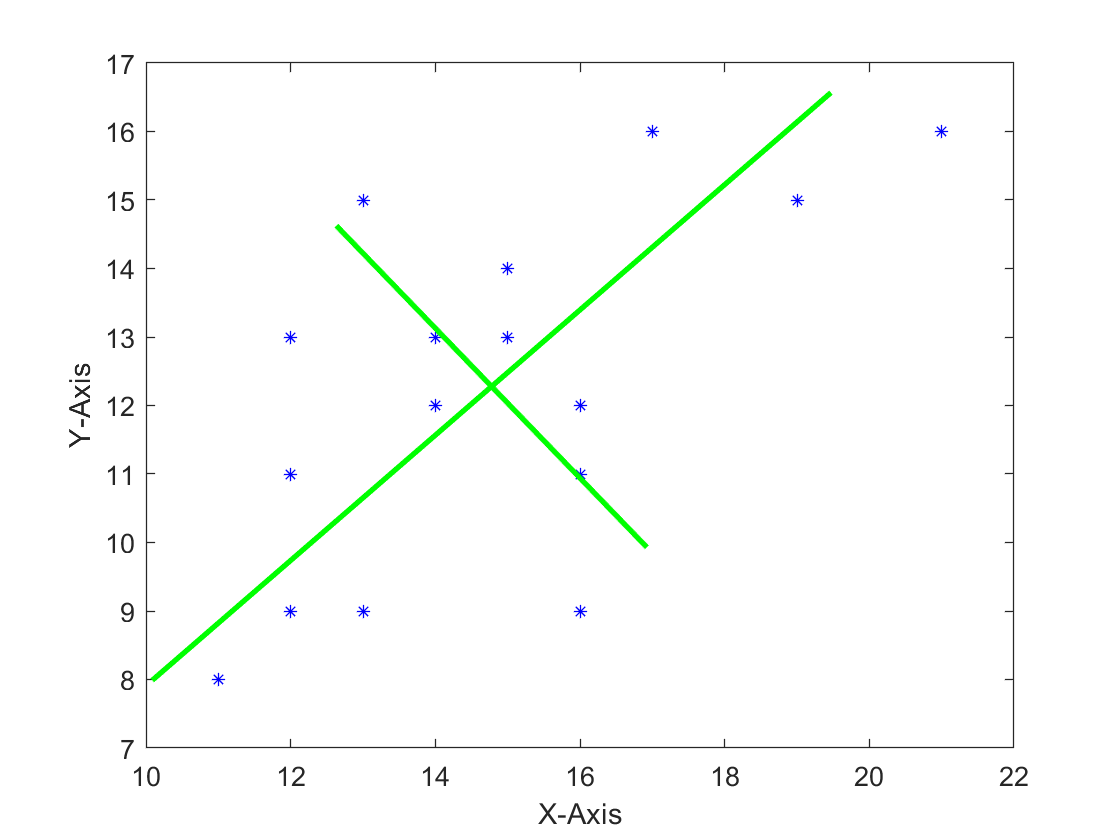
\includegraphics[scale=0.35 ]{Fig1.png}
%%		
%		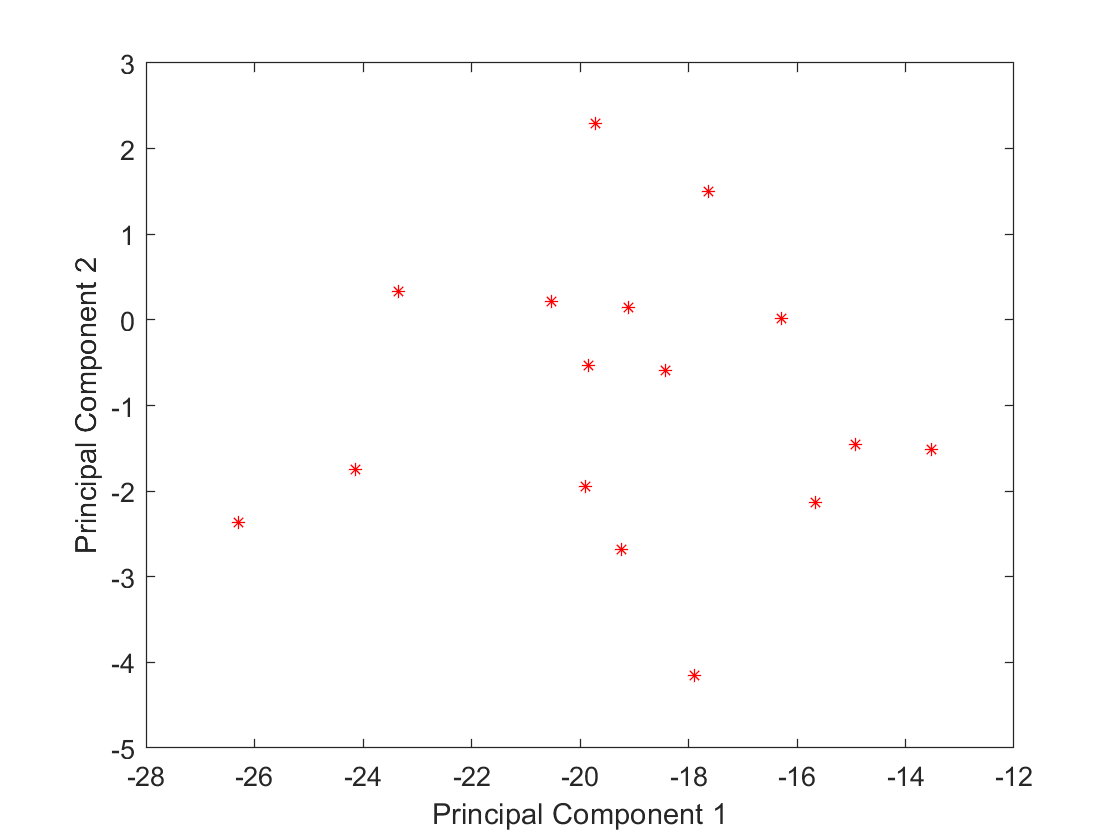
\includegraphics[scale=0.35 ]{Fig2.png}
%		\begin{center}
%			\begin{minipage}{.45\textwidth}
%				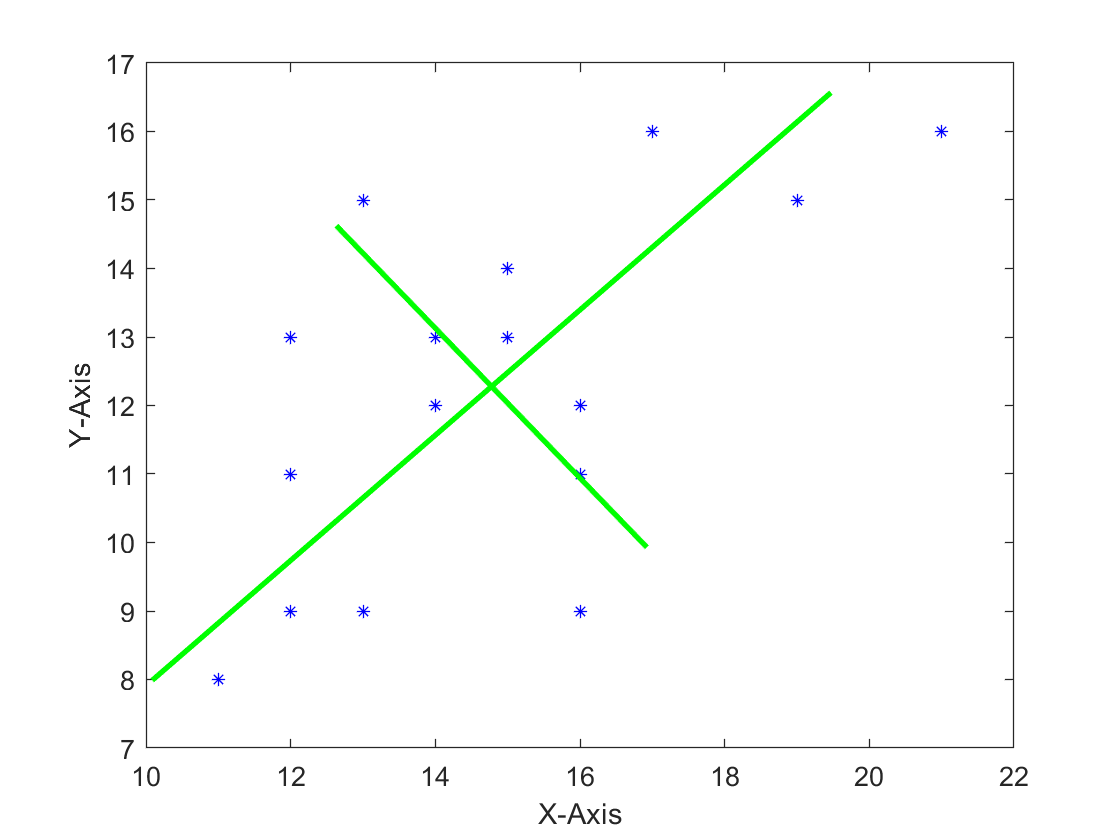
\includegraphics[scale=0.3]{Fig1.PNG}
%			\end{minipage}
%			\hspace*{.05\textwidth}
%			\begin{minipage}{.45\textwidth}
%				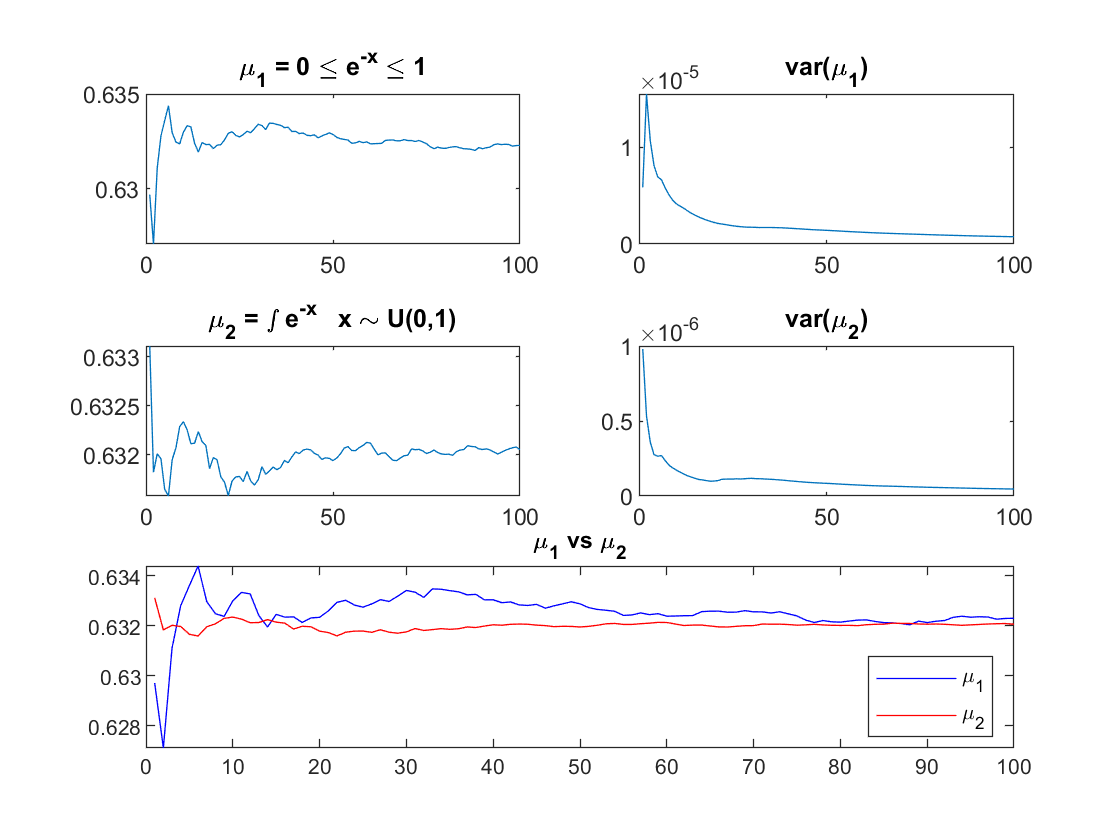
\includegraphics[scale=0.3]{Fig2.PNG}
%			\end{minipage}
%		\end{center}
	
\subsection*{Code:}
	\lstinputlisting[]{HW3.m}
	
\section*{Python (Problems 4-6)}
	
	\begin{Verbatim}[commandchars=\\\{\}]
	{\color{incolor}In [{\color{incolor}9}]:} \PY{c+c1}{\PYZsh{}Problem 4}
	\PY{l+s+s2}{\PYZdq{}}\PY{l+s+s2}{\PYZhy{}\PYZhy{}\PYZhy{}\PYZhy{}\PYZhy{}Problem 4\PYZhy{}\PYZhy{}\PYZhy{}\PYZhy{}\PYZhy{}}\PY{l+s+s2}{\PYZdq{}}
	\PY{k+kn}{from} \PY{n+nn}{numpy} \PY{k}{import} \PY{o}{*}
	\PY{n}{set\PYZus{}printoptions}\PY{p}{(}\PY{n}{precision}\PY{o}{=}\PY{l+m+mi}{4}\PY{p}{)}
	
	\PY{n}{X}\PY{o}{=}\PY{n}{mat}\PY{p}{(}\PY{l+s+s2}{\PYZdq{}}\PY{l+s+s2}{5. 0. 9. 3.; 3. 6. 8. 9.; 4. 4. 9. 6.; 0. 3. 1. 8.; 2. 8. 2. 3.}\PY{l+s+s2}{\PYZdq{}}\PY{p}{)}
	\PY{n}{y}\PY{o}{=}\PY{n}{mat}\PY{p}{(}\PY{l+s+s2}{\PYZdq{}}\PY{l+s+s2}{20. 17. 32. 10. 12.}\PY{l+s+s2}{\PYZdq{}}\PY{p}{)}\PY{o}{.}\PY{n}{T}
	
	\PY{k}{def} \PY{n+nf}{backsub}\PY{p}{(}\PY{n}{X}\PY{p}{,} \PY{n}{y}\PY{p}{)}\PY{p}{:}
	\PY{n}{l} \PY{o}{=} \PY{n}{shape}\PY{p}{(}\PY{n}{X}\PY{p}{)}  
	\PY{n}{n} \PY{o}{=} \PY{n}{l}\PY{p}{[}\PY{l+m+mi}{1}\PY{p}{]}
	\PY{n}{b} \PY{o}{=} \PY{n}{zeros}\PY{p}{(}\PY{p}{(}\PY{n}{n}\PY{p}{,}\PY{l+m+mi}{1}\PY{p}{)}\PY{p}{)}
	\PY{n}{b}\PY{p}{[}\PY{n}{n}\PY{o}{\PYZhy{}}\PY{l+m+mi}{1}\PY{p}{,} \PY{l+m+mi}{0}\PY{p}{]} \PY{o}{=} \PY{n}{y}\PY{p}{[}\PY{n}{n}\PY{o}{\PYZhy{}}\PY{l+m+mi}{1}\PY{p}{,} \PY{l+m+mi}{0}\PY{p}{]}\PY{o}{/}\PY{n}{X}\PY{p}{[}\PY{n}{n}\PY{o}{\PYZhy{}}\PY{l+m+mi}{1}\PY{p}{,} \PY{n}{n}\PY{o}{\PYZhy{}}\PY{l+m+mi}{1}\PY{p}{]}
	\PY{k}{for} \PY{n}{j} \PY{o+ow}{in} \PY{n+nb}{range}\PY{p}{(}\PY{n}{n}\PY{o}{\PYZhy{}}\PY{l+m+mi}{1}\PY{p}{,}\PY{l+m+mi}{0}\PY{p}{,}\PY{o}{\PYZhy{}}\PY{l+m+mi}{1}\PY{p}{)}\PY{p}{:}
	\PY{n}{b}\PY{p}{[}\PY{n}{j}\PY{o}{\PYZhy{}}\PY{l+m+mi}{1}\PY{p}{,}\PY{l+m+mi}{0}\PY{p}{]} \PY{o}{=} \PY{p}{(}\PY{n}{y}\PY{p}{[}\PY{n}{j}\PY{o}{\PYZhy{}}\PY{l+m+mi}{1}\PY{p}{,}\PY{l+m+mi}{0}\PY{p}{]} \PY{o}{\PYZhy{}} \PY{n}{dot}\PY{p}{(}\PY{n}{X}\PY{p}{[}\PY{n}{j}\PY{o}{\PYZhy{}}\PY{l+m+mi}{1}\PY{p}{,} \PY{n+nb}{range}\PY{p}{(}\PY{n}{j}\PY{p}{,}\PY{n}{n}\PY{p}{)}\PY{p}{]}\PY{p}{,} \PY{n}{b}\PY{p}{[}\PY{n+nb}{range}\PY{p}{(}\PY{n}{j}\PY{p}{,}\PY{n}{n}\PY{p}{)}\PY{p}{,}\PY{l+m+mi}{0}\PY{p}{]}\PY{p}{)}\PY{p}{)}\PY{o}{/}\PY{n}{X}\PY{p}{[}\PY{n}{j}\PY{o}{\PYZhy{}}\PY{l+m+mi}{1}\PY{p}{,} \PY{n}{j}\PY{o}{\PYZhy{}}\PY{l+m+mi}{1}\PY{p}{]}
	\PY{k}{return} \PY{n}{b}
	
	\PY{k}{def} \PY{n+nf}{house}\PY{p}{(}\PY{n}{x}\PY{p}{)}\PY{p}{:}
	\PY{n}{m} \PY{o}{=} \PY{n}{size}\PY{p}{(}\PY{n}{x}\PY{p}{)}
	\PY{n}{mu} \PY{o}{=} \PY{n}{linalg}\PY{o}{.}\PY{n}{norm}\PY{p}{(}\PY{n}{x}\PY{p}{)}
	\PY{n}{v} \PY{o}{=} \PY{n}{x}\PY{o}{.}\PY{n}{copy}\PY{p}{(}\PY{p}{)}
	\PY{k}{if} \PY{n}{mu} \PY{o}{!=} \PY{l+m+mi}{0}\PY{p}{:}
	\PY{n}{c} \PY{o}{=} \PY{n}{x}\PY{p}{[}\PY{l+m+mi}{0}\PY{p}{]} \PY{o}{+} \PY{n}{sign}\PY{p}{(}\PY{n}{x}\PY{p}{[}\PY{l+m+mi}{0}\PY{p}{]}\PY{p}{)}\PY{o}{*}\PY{n}{mu}
	\PY{n}{v}\PY{p}{[}\PY{l+m+mi}{1}\PY{p}{:}\PY{n}{m}\PY{o}{+}\PY{l+m+mi}{1}\PY{p}{]} \PY{o}{=} \PY{n}{v}\PY{p}{[}\PY{l+m+mi}{1}\PY{p}{:}\PY{n}{m}\PY{o}{+}\PY{l+m+mi}{1}\PY{p}{]}\PY{o}{/}\PY{n}{c}
	\PY{n}{v}\PY{p}{[}\PY{l+m+mi}{0}\PY{p}{]} \PY{o}{=} \PY{l+m+mi}{1}
	\PY{k}{return} \PY{n}{v}
	
	\PY{k}{def} \PY{n+nf}{rowhouse}\PY{p}{(}\PY{n}{X}\PY{p}{,}\PY{n}{v}\PY{p}{)}\PY{p}{:}
	\PY{n}{X} \PY{o}{=} \PY{n}{mat}\PY{p}{(}\PY{n}{X}\PY{p}{)}
	\PY{n}{v} \PY{o}{=} \PY{n}{mat}\PY{p}{(}\PY{n}{v}\PY{p}{)}
	\PY{n}{X} \PY{o}{=} \PY{n}{X} \PY{o}{\PYZhy{}} \PY{l+m+mi}{2}\PY{o}{*}\PY{n}{v}\PY{o}{*}\PY{n}{v}\PY{o}{.}\PY{n}{T}\PY{o}{/}\PY{p}{(}\PY{n}{v}\PY{o}{.}\PY{n}{T}\PY{o}{*}\PY{n}{v}\PY{p}{)}\PY{o}{*}\PY{n}{X}
	\PY{k}{return} \PY{n}{X}
	
	\PY{k}{def} \PY{n+nf}{householder}\PY{p}{(}\PY{n}{X0}\PY{p}{)}\PY{p}{:}
	\PY{n}{X} \PY{o}{=} \PY{n}{mat}\PY{p}{(}\PY{n}{X0}\PY{o}{.}\PY{n}{copy}\PY{p}{(}\PY{p}{)}\PY{p}{)}
	\PY{n}{m}\PY{p}{,} \PY{n}{n} \PY{o}{=} \PY{n}{shape}\PY{p}{(}\PY{n}{X}\PY{p}{)}
	\PY{n}{v} \PY{o}{=} \PY{n}{mat}\PY{p}{(}\PY{n}{zeros}\PY{p}{(}\PY{p}{(}\PY{n}{m}\PY{p}{,}\PY{l+m+mi}{1}\PY{p}{)}\PY{p}{)}\PY{p}{)}
	\PY{k}{for} \PY{n}{j} \PY{o+ow}{in} \PY{n+nb}{range}\PY{p}{(}\PY{l+m+mi}{1}\PY{p}{,} \PY{n}{n}\PY{o}{+}\PY{l+m+mi}{1}\PY{p}{)}\PY{p}{:}
	\PY{n}{v}\PY{p}{[}\PY{n}{j}\PY{o}{\PYZhy{}}\PY{l+m+mi}{1}\PY{p}{:}\PY{n}{m}\PY{p}{]} \PY{o}{=} \PY{n}{house}\PY{p}{(}\PY{n}{X}\PY{p}{[}\PY{n}{j}\PY{o}{\PYZhy{}}\PY{l+m+mi}{1}\PY{p}{:}\PY{n}{m}\PY{p}{,}\PY{n}{j}\PY{o}{\PYZhy{}}\PY{l+m+mi}{1}\PY{p}{]}\PY{p}{)}
	\PY{n}{X}\PY{p}{[}\PY{n}{j}\PY{o}{\PYZhy{}}\PY{l+m+mi}{1}\PY{p}{:}\PY{n}{m}\PY{p}{,}\PY{n}{j}\PY{o}{\PYZhy{}}\PY{l+m+mi}{1}\PY{p}{:}\PY{n}{n}\PY{p}{]} \PY{o}{=} \PY{n}{rowhouse}\PY{p}{(}\PY{n}{X}\PY{p}{[}\PY{n}{j}\PY{o}{\PYZhy{}}\PY{l+m+mi}{1}\PY{p}{:}\PY{n}{m}\PY{p}{,}\PY{n}{j}\PY{o}{\PYZhy{}}\PY{l+m+mi}{1}\PY{p}{:}\PY{n}{n}\PY{p}{]}\PY{p}{,} \PY{n}{v}\PY{p}{[}\PY{n}{j}\PY{o}{\PYZhy{}}\PY{l+m+mi}{1}\PY{p}{:}\PY{n}{m}\PY{p}{]}\PY{p}{)}
	\PY{k}{return} \PY{n}{X}
	
	\PY{k}{def} \PY{n+nf}{multilinreg}\PY{p}{(}\PY{n}{X0}\PY{p}{,}\PY{n}{y0}\PY{p}{)}\PY{p}{:}
	\PY{n}{X} \PY{o}{=} \PY{n}{X0}\PY{o}{.}\PY{n}{copy}\PY{p}{(}\PY{p}{)}
	\PY{n}{y} \PY{o}{=} \PY{n}{y0}\PY{o}{.}\PY{n}{copy}\PY{p}{(}\PY{p}{)}
	\PY{n}{m}\PY{p}{,} \PY{n}{n} \PY{o}{=} \PY{n}{shape}\PY{p}{(}\PY{n}{X0}\PY{p}{)}
	\PY{k}{for} \PY{n}{j} \PY{o+ow}{in} \PY{n+nb}{range}\PY{p}{(}\PY{l+m+mi}{1}\PY{p}{,}\PY{n}{n}\PY{o}{+}\PY{l+m+mi}{1}\PY{p}{)}\PY{p}{:}
	\PY{n}{v} \PY{o}{=} \PY{n}{house}\PY{p}{(}\PY{n}{X}\PY{p}{[}\PY{n}{j}\PY{o}{\PYZhy{}}\PY{l+m+mi}{1}\PY{p}{:}\PY{n}{m}\PY{p}{,}\PY{n}{j}\PY{o}{\PYZhy{}}\PY{l+m+mi}{1}\PY{p}{]}\PY{p}{)}
	\PY{n}{X}\PY{p}{[}\PY{n}{j}\PY{o}{\PYZhy{}}\PY{l+m+mi}{1}\PY{p}{:}\PY{n}{m}\PY{p}{,}\PY{n}{j}\PY{o}{\PYZhy{}}\PY{l+m+mi}{1}\PY{p}{:}\PY{n}{n}\PY{p}{]} \PY{o}{=} \PY{n}{rowhouse}\PY{p}{(}\PY{n}{X}\PY{p}{[}\PY{n}{j}\PY{o}{\PYZhy{}}\PY{l+m+mi}{1}\PY{p}{:}\PY{n}{m}\PY{p}{,}\PY{n}{j}\PY{o}{\PYZhy{}}\PY{l+m+mi}{1}\PY{p}{:}\PY{n}{n}\PY{p}{]}\PY{p}{,} \PY{n}{v}\PY{p}{)}
	\PY{n}{beta} \PY{o}{=} \PY{o}{\PYZhy{}}\PY{l+m+mf}{2.}\PY{o}{*}\PY{p}{(}\PY{n}{v}\PY{o}{.}\PY{n}{T}\PY{o}{*}\PY{n}{y}\PY{p}{[}\PY{n}{j}\PY{o}{\PYZhy{}}\PY{l+m+mi}{1}\PY{p}{:}\PY{n}{m}\PY{p}{]}\PY{p}{)}\PY{o}{/}\PY{p}{(}\PY{n}{v}\PY{o}{.}\PY{n}{T}\PY{o}{*}\PY{n}{v}\PY{p}{)}
	\PY{n}{y}\PY{p}{[}\PY{n}{j}\PY{o}{\PYZhy{}}\PY{l+m+mi}{1}\PY{p}{:}\PY{n}{m}\PY{p}{]} \PY{o}{=} \PY{n}{y}\PY{p}{[}\PY{n}{j}\PY{o}{\PYZhy{}}\PY{l+m+mi}{1}\PY{p}{:}\PY{n}{m}\PY{p}{]} \PY{o}{+} \PY{n}{v}\PY{o}{*}\PY{n}{beta}
	
	\PY{n}{b} \PY{o}{=} \PY{n}{backsub}\PY{p}{(}\PY{n}{X}\PY{p}{,}\PY{n}{y}\PY{p}{)}
	\PY{k}{return} \PY{n}{b}
	
	\PY{n+nb}{print}\PY{p}{(}\PY{l+s+s2}{\PYZdq{}}\PY{l+s+s2}{b=}\PY{l+s+s2}{\PYZdq{}}\PY{p}{)}
	\PY{n+nb}{print}\PY{p}{(}\PY{n}{multilinreg}\PY{p}{(}\PY{n}{X}\PY{p}{,}\PY{n}{y}\PY{p}{)}\PY{p}{)}
	\end{Verbatim}
	
	\begin{Verbatim}[commandchars=\\\{\}]
	b=
	[[2.4413]
	[0.3949]
	[0.9165]
	[0.7156]]
	
	\end{Verbatim}
	
	\begin{Verbatim}[commandchars=\\\{\}]
	{\color{incolor}In [{\color{incolor}12}]:} \PY{c+c1}{\PYZsh{}Problem 5}
	\PY{k+kn}{from} \PY{n+nn}{matplotlib} \PY{k}{import} \PY{n}{pyplot}
	\PY{k+kn}{import} \PY{n+nn}{scipy}
	\PY{n+nb}{print}\PY{p}{(}\PY{l+s+s2}{\PYZdq{}}\PY{l+s+s2}{\PYZhy{}\PYZhy{}\PYZhy{}\PYZhy{}\PYZhy{}Problem 5\PYZhy{}\PYZhy{}\PYZhy{}\PYZhy{}\PYZhy{}}\PY{l+s+s2}{\PYZdq{}}\PY{p}{)}
	\PY{n}{X}\PY{o}{=}\PY{n}{mat}\PY{p}{(}\PY{l+s+s2}{\PYZdq{}}\PY{l+s+s2}{15. 16. 12. 14. 13. 15. 16. 21. 12. 11. 19. 14. 13. 14. 16. 17. 12. 16.; 13. 11. 13. 12. 9. 14. 12. 16. 9. 8. 15. 13. 15. 13. 12. 16. 11. 9.}\PY{l+s+s2}{\PYZdq{}}\PY{p}{)}
	\PY{n+nb}{print}\PY{p}{(}\PY{l+s+s2}{\PYZdq{}}\PY{l+s+s2}{X=}\PY{l+s+s2}{\PYZdq{}}\PY{p}{)}
	\PY{n+nb}{print}\PY{p}{(}\PY{n}{X}\PY{p}{)}
	
	\PY{n}{x}\PY{o}{=}\PY{n}{X}
	
	\PY{c+c1}{\PYZsh{}Part a}
	\PY{n+nb}{print}\PY{p}{(}\PY{l+s+s2}{\PYZdq{}}\PY{l+s+s2}{\PYZhy{}\PYZhy{}\PYZhy{}\PYZhy{}\PYZhy{}Part (a)\PYZhy{}\PYZhy{}\PYZhy{}\PYZhy{}\PYZhy{}}\PY{l+s+s2}{\PYZdq{}}\PY{p}{)}
	
	\PY{c+c1}{\PYZsh{}\PYZsh{} plot the raw data}
	\PY{n}{pyplot}\PY{o}{.}\PY{n}{figure}\PY{p}{(}\PY{l+m+mi}{0}\PY{p}{)}
	\PY{n}{pyplot}\PY{o}{.}\PY{n}{plot}\PY{p}{(}\PY{n}{x}\PY{p}{[}\PY{l+m+mi}{0}\PY{p}{,}\PY{p}{:}\PY{p}{]}\PY{p}{,} \PY{n}{x}\PY{p}{[}\PY{l+m+mi}{1}\PY{p}{,}\PY{p}{:}\PY{p}{]}\PY{p}{,} \PY{l+s+s1}{\PYZsq{}}\PY{l+s+s1}{b*}\PY{l+s+s1}{\PYZsq{}}\PY{p}{)}
	\PY{n}{pyplot}\PY{o}{.}\PY{n}{xlabel}\PY{p}{(}\PY{l+s+s1}{\PYZsq{}}\PY{l+s+s1}{X\PYZhy{}Axis}\PY{l+s+s1}{\PYZsq{}}\PY{p}{)}
	\PY{n}{pyplot}\PY{o}{.}\PY{n}{ylabel}\PY{p}{(}\PY{l+s+s1}{\PYZsq{}}\PY{l+s+s1}{Y\PYZhy{}Axis}\PY{l+s+s1}{\PYZsq{}}\PY{p}{)}\PY{p}{;}
	\PY{n}{pyplot}\PY{o}{.}\PY{n}{show}\PY{p}{(}\PY{p}{)}
	
	\PY{c+c1}{\PYZsh{}Part b}
	\PY{n+nb}{print}\PY{p}{(}\PY{l+s+s2}{\PYZdq{}}\PY{l+s+s2}{\PYZhy{}\PYZhy{}\PYZhy{}\PYZhy{}\PYZhy{}Part (b)\PYZhy{}\PYZhy{}\PYZhy{}\PYZhy{}\PYZhy{}}\PY{l+s+s2}{\PYZdq{}}\PY{p}{)}
	\PY{c+c1}{\PYZsh{}\PYZsh{}\PYZsh{}\PYZsh{} Perform the PCA analysis \PYZsh{}\PYZsh{}\PYZsh{}}
	\PY{n}{m}\PY{p}{,} \PY{n}{n} \PY{o}{=} \PY{n}{shape}\PY{p}{(}\PY{n}{x}\PY{p}{)}
	\PY{n+nb}{print}\PY{p}{(}\PY{n}{m}\PY{p}{)}
	\PY{n+nb}{print}\PY{p}{(}\PY{n}{n}\PY{p}{)}
	
	\PY{c+c1}{\PYZsh{} 1. Compute sample covariance}
	\PY{n}{C} \PY{o}{=} \PY{n}{cov}\PY{p}{(}\PY{n}{x}\PY{p}{)}
	\PY{n+nb}{print}\PY{p}{(}\PY{l+s+s2}{\PYZdq{}}\PY{l+s+s2}{C=}\PY{l+s+s2}{\PYZdq{}}\PY{p}{)}
	\PY{n+nb}{print}\PY{p}{(}\PY{n}{C}\PY{p}{)}
	
	\PY{c+c1}{\PYZsh{} 2. SVD on C}
	\PY{n}{U}\PY{p}{,} \PY{n}{S}\PY{p}{,} \PY{n}{Vh} \PY{o}{=} \PY{n}{linalg}\PY{o}{.}\PY{n}{svd}\PY{p}{(}\PY{n}{C}\PY{p}{)}
	\PY{n}{V} \PY{o}{=} \PY{n}{Vh}\PY{o}{.}\PY{n}{T}
	
	\PY{c+c1}{\PYZsh{} 3. select the first 2 columns of U}
	\PY{n}{U1} \PY{o}{=} \PY{n}{U}\PY{p}{[}\PY{p}{:}\PY{p}{,}\PY{l+m+mi}{0}\PY{p}{:}\PY{l+m+mi}{2}\PY{p}{]}
	\PY{n+nb}{print}\PY{p}{(}\PY{l+s+s2}{\PYZdq{}}\PY{l+s+s2}{U1=}\PY{l+s+s2}{\PYZdq{}}\PY{p}{)}
	\PY{n+nb}{print}\PY{p}{(}\PY{n}{U1}\PY{p}{)}
	
	\PY{c+c1}{\PYZsh{} 4. Define Z }
	\PY{n}{Z} \PY{o}{=} \PY{n}{U1}\PY{o}{.}\PY{n}{T}\PY{o}{*}\PY{n}{x}\PY{p}{;}
	
	\PY{c+c1}{\PYZsh{}\PYZsh{} plot the transformed data}
	\PY{n}{pyplot}\PY{o}{.}\PY{n}{figure}\PY{p}{(}\PY{l+m+mi}{2}\PY{p}{)}
	\PY{n}{pyplot}\PY{o}{.}\PY{n}{plot}\PY{p}{(}\PY{n}{Z}\PY{p}{[}\PY{l+m+mi}{0}\PY{p}{,}\PY{p}{:}\PY{p}{]}\PY{p}{,} \PY{n}{Z}\PY{p}{[}\PY{l+m+mi}{1}\PY{p}{,}\PY{p}{:}\PY{p}{]}\PY{p}{,} \PY{l+s+s1}{\PYZsq{}}\PY{l+s+s1}{r*}\PY{l+s+s1}{\PYZsq{}}\PY{p}{)}
	\PY{n}{pyplot}\PY{o}{.}\PY{n}{axis}\PY{p}{(}\PY{p}{[}\PY{o}{\PYZhy{}}\PY{l+m+mi}{110}\PY{p}{,} \PY{o}{\PYZhy{}}\PY{l+m+mi}{85}\PY{p}{,} \PY{o}{\PYZhy{}}\PY{l+m+mi}{1}\PY{p}{,} \PY{l+m+mi}{6}\PY{p}{]}\PY{p}{)}
	\PY{n}{pyplot}\PY{o}{.}\PY{n}{axis}\PY{p}{(}\PY{l+s+s1}{\PYZsq{}}\PY{l+s+s1}{equal}\PY{l+s+s1}{\PYZsq{}}\PY{p}{)}
	\PY{n}{pyplot}\PY{o}{.}\PY{n}{xlabel}\PY{p}{(}\PY{l+s+s1}{\PYZsq{}}\PY{l+s+s1}{Principal Component 1}\PY{l+s+s1}{\PYZsq{}}\PY{p}{)}
	\PY{n}{pyplot}\PY{o}{.}\PY{n}{ylabel}\PY{p}{(}\PY{l+s+s1}{\PYZsq{}}\PY{l+s+s1}{Principal Component 2}\PY{l+s+s1}{\PYZsq{}}\PY{p}{)}
	
	\PY{c+c1}{\PYZsh{}\PYZsh{} add the principal directions}
	\PY{n}{pyplot}\PY{o}{.}\PY{n}{figure}\PY{p}{(}\PY{l+m+mi}{1}\PY{p}{)}
	\PY{n}{pyplot}\PY{o}{.}\PY{n}{plot}\PY{p}{(}\PY{n}{x}\PY{p}{[}\PY{l+m+mi}{0}\PY{p}{,}\PY{p}{:}\PY{p}{]}\PY{p}{,} \PY{n}{x}\PY{p}{[}\PY{l+m+mi}{1}\PY{p}{,}\PY{p}{:}\PY{p}{]}\PY{p}{,} \PY{l+s+s1}{\PYZsq{}}\PY{l+s+s1}{b*}\PY{l+s+s1}{\PYZsq{}}\PY{p}{)}
	\PY{n}{pyplot}\PY{o}{.}\PY{n}{xlabel}\PY{p}{(}\PY{l+s+s1}{\PYZsq{}}\PY{l+s+s1}{X\PYZhy{}Axis }\PY{l+s+s1}{\PYZsq{}}\PY{p}{)}
	\PY{n}{pyplot}\PY{o}{.}\PY{n}{ylabel}\PY{p}{(}\PY{l+s+s1}{\PYZsq{}}\PY{l+s+s1}{Y\PYZhy{}Axis }\PY{l+s+s1}{\PYZsq{}}\PY{p}{)}\PY{p}{;}
	\PY{n}{m\PYZus{}x} \PY{o}{=} \PY{n}{x}\PY{o}{.}\PY{n}{mean}\PY{p}{(}\PY{n}{axis}\PY{o}{=}\PY{l+m+mi}{1}\PY{p}{)}
	\PY{n}{TP1} \PY{o}{=} \PY{n}{array}\PY{p}{(}\PY{l+m+mi}{2}\PY{o}{*}\PY{n}{sqrt}\PY{p}{(}\PY{n}{S}\PY{p}{[}\PY{l+m+mi}{0}\PY{p}{]}\PY{p}{)}\PY{o}{*}\PY{n}{mat}\PY{p}{(}\PY{p}{[}\PY{o}{\PYZhy{}}\PY{n}{U}\PY{p}{[}\PY{l+m+mi}{0}\PY{p}{,} \PY{l+m+mi}{0}\PY{p}{]}\PY{p}{,} \PY{n}{U}\PY{p}{[}\PY{l+m+mi}{0}\PY{p}{,} \PY{l+m+mi}{0}\PY{p}{]}\PY{p}{]}\PY{p}{)}\PY{o}{+}\PY{n}{m\PYZus{}x}\PY{p}{[}\PY{l+m+mi}{0}\PY{p}{]}\PY{p}{)}
	\PY{n}{TP2} \PY{o}{=} \PY{n}{array}\PY{p}{(}\PY{l+m+mi}{2}\PY{o}{*}\PY{n}{sqrt}\PY{p}{(}\PY{n}{S}\PY{p}{[}\PY{l+m+mi}{0}\PY{p}{]}\PY{p}{)}\PY{o}{*}\PY{n}{mat}\PY{p}{(}\PY{p}{[}\PY{o}{\PYZhy{}}\PY{n}{U}\PY{p}{[}\PY{l+m+mi}{1}\PY{p}{,} \PY{l+m+mi}{0}\PY{p}{]}\PY{p}{,} \PY{n}{U}\PY{p}{[}\PY{l+m+mi}{1}\PY{p}{,} \PY{l+m+mi}{0}\PY{p}{]}\PY{p}{]}\PY{p}{)}\PY{o}{+}\PY{n}{m\PYZus{}x}\PY{p}{[}\PY{l+m+mi}{1}\PY{p}{]}\PY{p}{)}
	\PY{n}{TP3} \PY{o}{=} \PY{n}{array}\PY{p}{(}\PY{l+m+mi}{2}\PY{o}{*}\PY{n}{sqrt}\PY{p}{(}\PY{n}{S}\PY{p}{[}\PY{l+m+mi}{1}\PY{p}{]}\PY{p}{)}\PY{o}{*}\PY{n}{mat}\PY{p}{(}\PY{p}{[}\PY{o}{\PYZhy{}}\PY{n}{U}\PY{p}{[}\PY{l+m+mi}{0}\PY{p}{,} \PY{l+m+mi}{1}\PY{p}{]}\PY{p}{,} \PY{n}{U}\PY{p}{[}\PY{l+m+mi}{0}\PY{p}{,} \PY{l+m+mi}{1}\PY{p}{]}\PY{p}{]}\PY{p}{)}\PY{o}{+}\PY{n}{m\PYZus{}x}\PY{p}{[}\PY{l+m+mi}{0}\PY{p}{]}\PY{p}{)}
	\PY{n}{TP4} \PY{o}{=} \PY{n}{array}\PY{p}{(}\PY{l+m+mi}{2}\PY{o}{*}\PY{n}{sqrt}\PY{p}{(}\PY{n}{S}\PY{p}{[}\PY{l+m+mi}{1}\PY{p}{]}\PY{p}{)}\PY{o}{*}\PY{n}{mat}\PY{p}{(}\PY{p}{[}\PY{o}{\PYZhy{}}\PY{n}{U}\PY{p}{[}\PY{l+m+mi}{1}\PY{p}{,} \PY{l+m+mi}{1}\PY{p}{]}\PY{p}{,} \PY{n}{U}\PY{p}{[}\PY{l+m+mi}{1}\PY{p}{,} \PY{l+m+mi}{1}\PY{p}{]}\PY{p}{]}\PY{p}{)}\PY{o}{+}\PY{n}{m\PYZus{}x}\PY{p}{[}\PY{l+m+mi}{1}\PY{p}{]}\PY{p}{)}      
	\PY{n}{pyplot}\PY{o}{.}\PY{n}{plot}\PY{p}{(}\PY{n}{TP1}\PY{p}{[}\PY{l+m+mi}{0}\PY{p}{]}\PY{p}{,} \PY{n}{TP2}\PY{p}{[}\PY{l+m+mi}{0}\PY{p}{]}\PY{p}{,} \PY{l+s+s1}{\PYZsq{}}\PY{l+s+s1}{g\PYZhy{}}\PY{l+s+s1}{\PYZsq{}}\PY{p}{)}
	\PY{n}{pyplot}\PY{o}{.}\PY{n}{plot}\PY{p}{(}\PY{n}{TP3}\PY{p}{[}\PY{l+m+mi}{0}\PY{p}{]}\PY{p}{,} \PY{n}{TP4}\PY{p}{[}\PY{l+m+mi}{0}\PY{p}{]}\PY{p}{,} \PY{l+s+s1}{\PYZsq{}}\PY{l+s+s1}{g\PYZhy{}}\PY{l+s+s1}{\PYZsq{}}\PY{p}{)}  
	
	\PY{n}{pyplot}\PY{o}{.}\PY{n}{show}\PY{p}{(}\PY{p}{)}
	
	\PY{c+c1}{\PYZsh{}\PYZsh{} compare the covariance and the total variance}
	\PY{n}{Cov\PYZus{}x} \PY{o}{=} \PY{n}{cov}\PY{p}{(}\PY{n}{x}\PY{p}{)}
	\PY{n}{Cov\PYZus{}Z} \PY{o}{=} \PY{n}{cov}\PY{p}{(}\PY{n}{Z}\PY{p}{)}
	\PY{n}{Total\PYZus{}var\PYZus{}x} \PY{o}{=} \PY{n}{trace}\PY{p}{(}\PY{n}{Cov\PYZus{}x}\PY{p}{)}
	\PY{n}{Total\PYZus{}var\PYZus{}Z} \PY{o}{=} \PY{n}{trace}\PY{p}{(}\PY{n}{Cov\PYZus{}Z}\PY{p}{)}
	\PY{n}{Ratio}\PY{o}{=}\PY{n}{Total\PYZus{}var\PYZus{}x}\PY{o}{/}\PY{n}{Total\PYZus{}var\PYZus{}Z}
	
	\PY{c+c1}{\PYZsh{}print(\PYZsq{}total\PYZus{}var\PYZus{}x = \PYZsq{} + repr(Total\PYZus{}var\PYZus{}x), \PYZsq{}total\PYZus{}var\PYZus{}z = \PYZsq{} + repr(Total\PYZus{}var\PYZus{}Z))}
	
	\PY{n+nb}{print}\PY{p}{(}\PY{l+s+s1}{\PYZsq{}}\PY{l+s+s1}{total\PYZus{}var\PYZus{}x = }\PY{l+s+si}{\PYZpc{}5.2f}\PY{l+s+s1}{\PYZsq{}} \PY{o}{\PYZpc{}}\PY{k}{Total\PYZus{}var\PYZus{}x}, \PYZsq{}total\PYZus{}var\PYZus{}Z = \PYZpc{}5.2f\PYZsq{} \PYZpc{}Total\PYZus{}var\PYZus{}Z, \PYZsq{}Ratio is: \PYZpc{}2.4f\PYZsq{} \PYZpc{}Ratio) 
	\end{Verbatim}
	
	\begin{Verbatim}[commandchars=\\\{\}]
	-----Problem 5-----
	X=
	[[15. 16. 12. 14. 13. 15. 16. 21. 12. 11. 19. 14. 13. 14. 16. 17. 12. 16.]
	[13. 11. 13. 12.  9. 14. 12. 16.  9.  8. 15. 13. 15. 13. 12. 16. 11.  9.]]
	-----Part (a)-----
	
	\end{Verbatim}
	
	\begin{center}
		\adjustimage{max size={0.9\linewidth}{0.9\paperheight}}{output_1_1.png}
	\end{center}
	{ \hspace*{\fill} \\}
	
	\begin{Verbatim}[commandchars=\\\{\}]
	-----Part (b)-----
	2
	18
	C=
	[[6.6536 3.7712]
	[3.7712 5.9771]]
	U1=
	[[-0.738  -0.6748]
	[-0.6748  0.738 ]]
	
	\end{Verbatim}
	
	\begin{center}
		\adjustimage{max size={0.9\linewidth}{0.9\paperheight}}{output_1_3.png}
	\end{center}
	{ \hspace*{\fill} \\}
	
	\begin{center}
		\adjustimage{max size={0.9\linewidth}{0.9\paperheight}}{output_1_4.png}
	\end{center}
	{ \hspace*{\fill} \\}
	
	\begin{Verbatim}[commandchars=\\\{\}]
	total\_var\_x = 12.63 total\_var\_Z = 12.63 Ratio is: 1.0000
	
	\end{Verbatim}
	
	\begin{Verbatim}[commandchars=\\\{\}]
	{\color{incolor}In [{\color{incolor}9}]:} \PY{c+c1}{\PYZsh{}Problem 5}
	\PY{n+nb}{print}\PY{p}{(}\PY{l+s+s2}{\PYZdq{}}\PY{l+s+s2}{\PYZhy{}\PYZhy{}\PYZhy{}\PYZhy{}\PYZhy{}Problem 5\PYZhy{}\PYZhy{}\PYZhy{}\PYZhy{}\PYZhy{}}\PY{l+s+s2}{\PYZdq{}}\PY{p}{)}
	\PY{n}{set\PYZus{}printoptions}\PY{p}{(}\PY{n}{precision}\PY{o}{=}\PY{l+m+mi}{4}\PY{p}{)}
	
	\PY{c+c1}{\PYZsh{}Importing Data}
	\PY{k+kn}{import} \PY{n+nn}{scipy}\PY{n+nn}{.}\PY{n+nn}{io}
	\PY{n}{mat\PYZus{}contents} \PY{o}{=} \PY{n}{scipy}\PY{o}{.}\PY{n}{io}\PY{o}{.}\PY{n}{loadmat}\PY{p}{(}\PY{l+s+s1}{\PYZsq{}}\PY{l+s+s1}{hw3\PYZus{}3\PYZus{}data.mat}\PY{l+s+s1}{\PYZsq{}}\PY{p}{)}
	\PY{n}{X} \PY{o}{=} \PY{n}{mat}\PY{p}{(}\PY{n}{mat\PYZus{}contents}\PY{p}{[}\PY{l+s+s1}{\PYZsq{}}\PY{l+s+s1}{X}\PY{l+s+s1}{\PYZsq{}}\PY{p}{]}\PY{p}{)}
	\PY{n}{y} \PY{o}{=} \PY{n}{mat}\PY{p}{(}\PY{n}{mat\PYZus{}contents}\PY{p}{[}\PY{l+s+s1}{\PYZsq{}}\PY{l+s+s1}{y}\PY{l+s+s1}{\PYZsq{}}\PY{p}{]}\PY{p}{)}
	
	\PY{c+c1}{\PYZsh{}Part a}
	\PY{n+nb}{print}\PY{p}{(}\PY{l+s+s2}{\PYZdq{}}\PY{l+s+s2}{\PYZhy{}\PYZhy{}\PYZhy{}\PYZhy{}Part a\PYZhy{}\PYZhy{}\PYZhy{}\PYZhy{}}\PY{l+s+s2}{\PYZdq{}}\PY{p}{)}
	
	\PY{c+c1}{\PYZsh{}\PYZsh{}\PYZsh{}\PYZsh{} Perform the PCA analysis \PYZsh{}\PYZsh{}\PYZsh{}}
	\PY{n}{m}\PY{p}{,} \PY{n}{n} \PY{o}{=} \PY{n}{shape}\PY{p}{(}\PY{n}{X}\PY{p}{)}
	\PY{n+nb}{print}\PY{p}{(}\PY{l+s+s1}{\PYZsq{}}\PY{l+s+s1}{X\PYZhy{}m=}\PY{l+s+s1}{\PYZsq{}}\PY{p}{,} \PY{n}{m}\PY{p}{,} \PY{l+s+s1}{\PYZsq{}}\PY{l+s+s1}{X\PYZhy{}n=}\PY{l+s+s1}{\PYZsq{}}\PY{p}{,} \PY{n}{n}\PY{p}{)} \PY{c+c1}{\PYZsh{}200x200}
	
	\PY{c+c1}{\PYZsh{} i. Compute sample covariance}
	\PY{n}{C} \PY{o}{=} \PY{n}{cov}\PY{p}{(}\PY{n}{X}\PY{o}{.}\PY{n}{T}\PY{p}{)}
	\PY{n}{a}\PY{p}{,} \PY{n}{b} \PY{o}{=} \PY{n}{shape}\PY{p}{(}\PY{n}{C}\PY{p}{)}
	\PY{n+nb}{print}\PY{p}{(}\PY{l+s+s1}{\PYZsq{}}\PY{l+s+s1}{C\PYZhy{}m=}\PY{l+s+s1}{\PYZsq{}}\PY{p}{,} \PY{n}{a}\PY{p}{,} \PY{l+s+s1}{\PYZsq{}}\PY{l+s+s1}{C\PYZhy{}n=}\PY{l+s+s1}{\PYZsq{}}\PY{p}{,} \PY{n}{b}\PY{p}{)} \PY{c+c1}{\PYZsh{}100x100}
	
	\PY{c+c1}{\PYZsh{} ii. SVD on C}
	\PY{n}{U}\PY{p}{,} \PY{n}{S}\PY{p}{,} \PY{n}{Vh} \PY{o}{=} \PY{n}{linalg}\PY{o}{.}\PY{n}{svd}\PY{p}{(}\PY{n}{C}\PY{p}{)}
	\PY{n}{V} \PY{o}{=} \PY{n}{Vh}\PY{o}{.}\PY{n}{T}
	
	\PY{c+c1}{\PYZsh{} iii. select the first D=10 U}
	\PY{n}{U1} \PY{o}{=} \PY{n}{V}\PY{p}{[}\PY{p}{:}\PY{p}{,}\PY{l+m+mi}{0}\PY{p}{:}\PY{l+m+mi}{10}\PY{p}{]}
	\PY{n}{o}\PY{p}{,} \PY{n}{p} \PY{o}{=} \PY{n}{shape}\PY{p}{(}\PY{n}{U1}\PY{p}{)}
	\PY{n+nb}{print}\PY{p}{(}\PY{l+s+s1}{\PYZsq{}}\PY{l+s+s1}{C\PYZhy{}m=}\PY{l+s+s1}{\PYZsq{}}\PY{p}{,} \PY{n}{o}\PY{p}{,} \PY{l+s+s1}{\PYZsq{}}\PY{l+s+s1}{C\PYZhy{}n=}\PY{l+s+s1}{\PYZsq{}}\PY{p}{,} \PY{n}{p}\PY{p}{)} \PY{c+c1}{\PYZsh{}100x10}
	
	\PY{c+c1}{\PYZsh{} iv. Define X3 (Prompt\PYZsq{}s X1) }
	\PY{n}{X3} \PY{o}{=} \PY{n}{X}\PY{o}{*}\PY{n}{U1}\PY{p}{;}
	\PY{n}{q}\PY{p}{,} \PY{n}{r} \PY{o}{=} \PY{n}{shape}\PY{p}{(}\PY{n}{X3}\PY{p}{)}
	\PY{n+nb}{print}\PY{p}{(}\PY{l+s+s1}{\PYZsq{}}\PY{l+s+s1}{X3\PYZhy{}m=}\PY{l+s+s1}{\PYZsq{}}\PY{p}{,} \PY{n}{q}\PY{p}{,} \PY{l+s+s1}{\PYZsq{}}\PY{l+s+s1}{X3\PYZhy{}n=}\PY{l+s+s1}{\PYZsq{}}\PY{p}{,} \PY{n}{r}\PY{p}{)} \PY{c+c1}{\PYZsh{}200x10}
	
	
	\PY{c+c1}{\PYZsh{}Part b}
	\PY{n+nb}{print}\PY{p}{(}\PY{l+s+s2}{\PYZdq{}}\PY{l+s+s2}{\PYZhy{}\PYZhy{}\PYZhy{}\PYZhy{}Part b\PYZhy{}\PYZhy{}\PYZhy{}\PYZhy{}}\PY{l+s+s2}{\PYZdq{}}\PY{p}{)}
	\PY{n}{b}\PY{o}{=}\PY{n}{multilinreg}\PY{p}{(}\PY{n}{X3}\PY{p}{,}\PY{n}{y}\PY{p}{)}
	\PY{n+nb}{print}\PY{p}{(}\PY{l+s+s1}{\PYZsq{}}\PY{l+s+s1}{b=}\PY{l+s+s1}{\PYZsq{}}\PY{p}{)}
	\PY{n+nb}{print}\PY{p}{(}\PY{n}{b}\PY{p}{)}
	
	\PY{c+c1}{\PYZsh{}Part c}
	\PY{n+nb}{print}\PY{p}{(}\PY{l+s+s2}{\PYZdq{}}\PY{l+s+s2}{\PYZhy{}\PYZhy{}\PYZhy{}\PYZhy{}Part c\PYZhy{}\PYZhy{}\PYZhy{}\PYZhy{}}\PY{l+s+s2}{\PYZdq{}}\PY{p}{)}
	\PY{n}{E}\PY{o}{=}\PY{n}{y}\PY{o}{\PYZhy{}}\PY{n}{X3}\PY{o}{*}\PY{n}{b}
	\PY{n+nb}{print}\PY{p}{(}\PY{l+s+s2}{\PYZdq{}}\PY{l+s+s2}{SSE = }\PY{l+s+s2}{\PYZdq{}}\PY{p}{,}\PY{n}{linalg}\PY{o}{.}\PY{n}{norm}\PY{p}{(}\PY{n}{E}\PY{p}{)}\PY{p}{)}
	\end{Verbatim}
	
	\begin{Verbatim}[commandchars=\\\{\}]
	-----Problem 5-----
	----Part a----
	X-m= 200 X-n= 100
	C-m= 100 C-n= 100
	C-m= 100 C-n= 10
	X3-m= 200 X3-n= 10
	----Part b----
	b=
	[[ 1.0742]
	[-1.7688]
	[ 0.104 ]
	[ 0.3633]
	[-0.3864]
	[ 0.4965]
	[ 0.8623]
	[ 1.3953]
	[-0.0185]
	[ 1.0064]]
	----Part c----
	SSE =  33.628167484025035
	
	\end{Verbatim}
\end{document}
